\chapter{Второй раздел, посвященный тому, как делать рисунки и формулы}
\label{ch:chap2}

\section{Рисунки}
\label{sec:fig}

\subsection{Обычные одинарные рисунки, управление размером, подписями и ссылками в тексте}
\label{subsec:simp-fig}

Рисунки в \LaTeX{} нумеруются автоматически. Если мы задали им уникальные метки, то мы можем к ним потом также обращаться. Ссылки на рисунки в тексте, также как ссылки на разделы и библиографические записи, кликабельные. Например, на \hyperref[fig:bird1]{Рисунке \ref*{fig:bird1}} представлена некоторая неизвестная нам птица. По умолчанию размер рисунков будет продгоняться под ширину текста, но в среде \verb|figure| можно установить ширину вручную. Например, тут ширина установлена в половину от ширины текста. Подписи к рисункам сделаны по ГОСТ: в центре, без точки в конце, есть полнотекстовая надпись "<Рисунок"> и длинное тире в качестве разделителя. Шрифт подписи сделан меньше основнового текстового шрифта (12 кегль). Так выглядит аккуратнее, а ГОСТ это, вроде бы, не запрещает.

    \begin{figure}[ht]
        \centering
        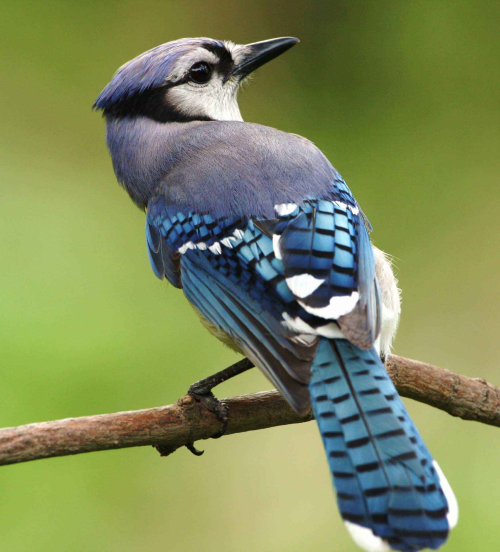
\includegraphics[width=0.5\textwidth]{bird1}
        \caption{Это типа какая-то птица}
        \label{fig:bird1}
    \end{figure}

Теперь продемонстрируем, как будут выглядеть длинные многострочные подписи. Для этого посмотрим на вторую неизвестную нам птицу, представленную на \hyperref[fig:bird2]{Рисунке \ref*{fig:bird2}}. Кстати, тут задан другой размер рисунка --- одна третья от ширины страницы.

    \begin{figure}[ht]
        \centering
        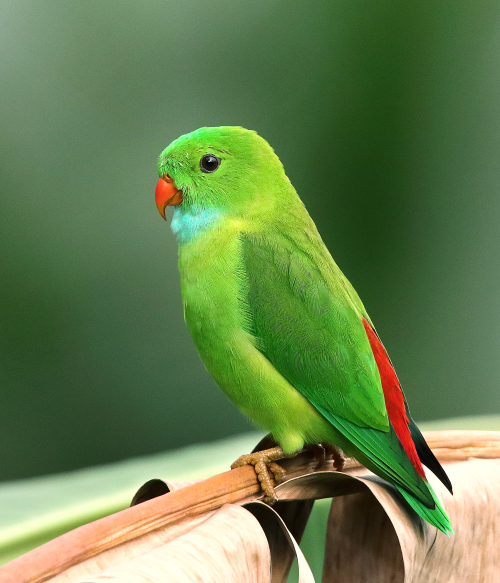
\includegraphics[width=0.33\textwidth]{bird2}
        \caption{Это другая птица, которая отличается от первой птицы формой клюва, цветом оперения, ареалом обитания, а также умением повторять за своим владельцем. Последнее, однако, не точно: птица, конечно, похожа на папугая, но мы не можем знать наверняка}
        \label{fig:bird2}
    \end{figure}

Мы напишем тут какой-нибудь текст, чтобы было видно величину отступа после подписи к рисунку. Мы не меняли это значение, оставили то, которое установлены в данном классе по умолчанию.

\subsection{Сложные многоуровневые рисунки}
\label{subsec:comp-fig}

Теперь посмотрим на то, как делать сложные рисунки. Обычно речь идет о двух-трех-четырех подрисунках, которые нумеруют (а), (б) и так далее. Мы делаем это при помощи среды \verb|subfigure| и инструментов, которые нам дает пакет \verb|subcaption|. На примере \hyperref[fig:tiger]{Рисунка \ref*{fig:tiger}} посмотрим, как задавать геометрию и расположение рисунков. Здесь два изображения разного формата, поэтому мы вручную выровняли их по высоте.

\begin{figure}[ht]
	\centering
\hspace*{\fill}%
	\begin{subfigure}[b]{0.49\textwidth}
        \centering
		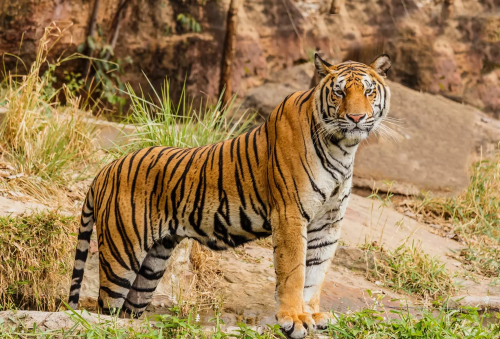
\includegraphics[height=5cm,keepaspectratio]{tiger1}
		\caption{}
		\label{fig:tiger1}
	\end{subfigure}
\hfill
	\begin{subfigure}[b]{0.49\textwidth}
        \centering
		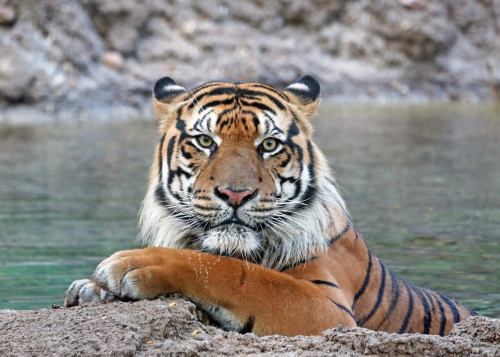
\includegraphics[height=5cm,keepaspectratio]{tiger2}
        \caption{}
		\label{fig:tiger2}
	\end{subfigure}
\hspace*{\fill}%
	\caption{Тигры. На рисунке (а) представлен гуляющий в саванне тигр, а на рисунке \\ (б) --- купающийся в водоеме. Тигр на (б) выглядит весьма довольным}
	\label{fig:tiger}
\end{figure}

Обратите внимание, что при помощи уже известных нам инструмеров можно обращаться не только в целом к рисункам, но и к конкретным подрисункам. Например, отметим, насколько же мощны лапищи этого прекрасного тигра на \hyperref[fig:tiger2]{Рисунке \ref*{fig:tiger2}}. Далее мы посмотрим, как делать двухэтажные рисунки. Добавим еще один рисунок внизу по центру. \LaTeX{} может сам менять местами рисунки и окружающий их текст с целью избежать пустых мест на страницах.

\begin{figure}[!ht]
	\centering
\hspace*{\fill}%
	\begin{subfigure}[b]{0.33\textwidth}
        \centering
		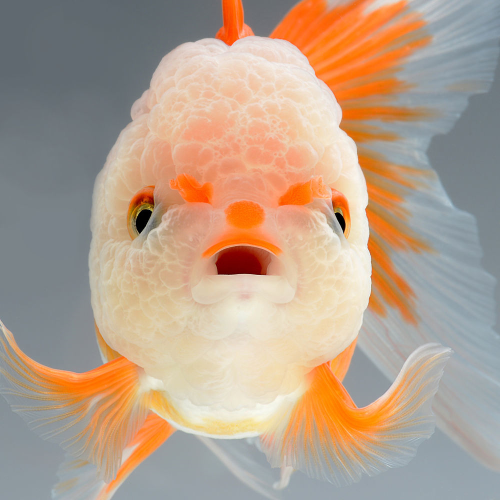
\includegraphics{fish1}
		\caption{}
		\label{fig:fish1}
	\end{subfigure}
\hfill
	\begin{subfigure}[b]{0.33\textwidth}
        \centering
		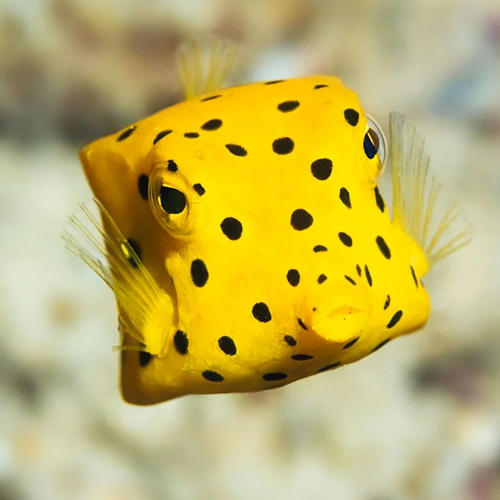
\includegraphics{fish2}
        \caption{}
		\label{fig:fish2}
	\end{subfigure}
\hspace*{\fill}%
\par\vspace{\abovecaptionskip}
        \begin{subfigure}[b]{0.33\textwidth}
        \centering
		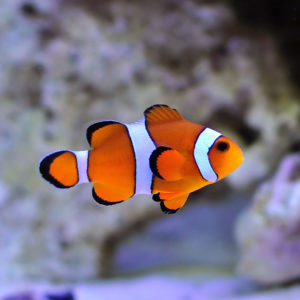
\includegraphics{fish3}
		\caption{}
		\label{fig:fish3}
	\end{subfigure}
	\caption{Разные рыбы}
	\label{fig:fish}
\end{figure}

На \hyperref[fig:fish]{Рисунке \ref*{fig:fish}} есть три фотографии одинакового размера, причем третья находится в нижнем ряду по центру. Нехитрым образом можем также сделать ссылку, которая обращается будто бы сразу к нескольким подрисункам, хотя в действительности ведет на весь рисунок. Например, можем написать так: \hyperref[fig:fish]{Рисунок \ref*{fig:fish}а--в}.

\section{Формулы}
\label{sec:equ}

Тут все просто, можете погуглить, как делать формулы, какие пакеты надо для этого подгружать, и т.д. Формулы можно вставлять прямо в текст, это делается при помощи одинарных знаков \verb|$|. Например, можно сделать вот такую штуку: $x = \frac{-b \pm \sqrt{b^2-4ac}}{2a}$. На такие формулы неудобно ссылаться. Можно сделать формулу на отдельной строке, присвоить ей номер и метку, чтобы потом обращаться к этой формуле из любого места в тексте при помощи уже известной нам команд \verb|ref| и \verb|hyperref|. Для этого есть среда \verb|equation|. Запишем выражение:
\begin{equation}
\label{eq:e1}
\frac{n!}{k!(n-k)!} = \binom{n}{k}.
\end{equation}
После этого в тексте можно ссылаться точно так же на Выражение \ref{eq:e1}, что часто оказывается весьма полезно. Можно использовать и \verb|hyperref|, сделав ссылку на \hyperref[eq:e1]{Выражение \ref*{eq:e1}} --- выбирайте сами.

Кстати, можно еще делать красивые химические реакции. В качестве примера рассмотрим \hyperref[eq:e2]{Выражение \ref*{eq:e2}}. Для создания таких выражений используется пакет \verb|mhchem|.
\begin{equation}
    \label{eq:e2}
    \ce{Na2SO4 ->[H2O] Na+ + SO4^2-}.
\end{equation}

\endinput